\documentclass{article}

\usepackage{amsfonts, amsmath, amsthm}
\usepackage[letterpaper, total={6in, 9in}]{geometry}
% \usepackage[noend]{algorithmic}
\usepackage[vlined,ruled,linesnumbered]{algorithm2e}
\usepackage{float}
\usepackage{caption}

%% preamble packages and symbols
%!TEX root = main.tex

% LC: debug
%==========================================================================
%\usepackage{refcheck}
%\usepackage[notref]{showkeys}
%==========================================================================

% LC: to be used for TRO
%==========================================================================
% \usepackage{mathptmx} % assumes new font selection scheme installed
%\usepackage{times} % assumes new font selection scheme installed
%==========================================================================
\usepackage{comment}
\usepackage{siunitx}
\usepackage{relsize}
\usepackage{ifthen}
\usepackage[colorinlistoftodos]{todonotes}

\usepackage[caption=false]{subfig}

% \begin{comment}
% % Fancy formatting 
% \usepackage[tracking=false,kerning=true,spacing=true]{microtype}
% \usepackage[caption=false]{subfig}

% % \DeclareFieldFormat[article]{pages}{#1}%
% % \DeclareFieldFormat[inproceedings]{pages}{#1}%

\usepackage[backend=biber,style=numeric,sorting=none,backref=true]{biblatex}
\addbibresource{refs.bib}

% \usepackage[noadjust]{cite}
\usepackage[vlined,ruled,linesnumbered]{algorithm2e}
\usepackage{graphics} % for pdf, bitmapped graphics files
\usepackage{rotating}
\usepackage{color}
\usepackage{enumerate}
\usepackage[T1]{fontenc}
\usepackage{psfrag}
\usepackage{epsfig} % for postscript graphics files
%\usepackage{subfigure}
% \usepackage{hyperref}
\usepackage{booktabs}
\usepackage{graphicx,url}
\usepackage{multirow}
\usepackage{array}
\usepackage{latexsym}
\usepackage{amsfonts}
\usepackage{amsmath}
\usepackage{amssymb}
\usepackage{mathtools}
%\usepackage{amsthm}
\usepackage{xstring}
\usepackage{multirow}
\usepackage{xcolor}
\usepackage{prettyref}
\usepackage{flexisym}
\usepackage{bigdelim}
\usepackage{breqn} % load this last
\usepackage{listings}
\let\labelindent\relax
\usepackage{enumitem}
\usepackage{xspace}
\usepackage{bm}
\graphicspath{{./figures/}}
\usepackage{tikz}
\usetikzlibrary{matrix,calc}


%\usepackage{ifpdf}
% Heiko Oberdiek's ifpdf.sty is very useful if you need conditional
% compilation based on whether the output is pdf or dvi.
% usage:
% \ifpdf
%   % pdf code
% \else
%    dvi code
% \fi
% The latest version of ifpdf.sty can be obtained from:
% http://www.ctan.org/tex-archive/macros/latex/contrib/oberdiek/
% Also, note that IEEEtran.cls V1.7 and later provides a builtin
% \ifCLASSINFOpdf conditional that works the same way.
% When switching from latex to pdflatex and vice-versa, the compiler may
% have to be run twice to clear warning/error messages.

% *** GRAPHICS RELATED PACKAGES ***
%
%\ifCLASSINFOpdf
  % \usepackage[pdftex]{graphicx}
  % declare the path(s) where your graphic files are
  % \graphicspath{{../pdf/}{../jpeg/}}
  % and their extensions so you won't have to specify these with
  % every instance of \includegraphics
  % \DeclareGraphicsExtensions{.pdf,.jpeg,.png}
%\else
  % or other class option (dvipsone, dvipdf, if not using dvips). graphicx
  % will default to the driver specified in the system graphics.cfg if no
  % driver is specified.
  % \usepackage[dvips]{graphicx}
  % declare the path(s) where your graphic files are
  % \graphicspath{{../eps/}}
  % and their extensions so you won't have to specify these with
  % every instance of \includegraphics
  % \DeclareGraphicsExtensions{.eps}
%\fi


\usepackage{mdwlist}
\let\stditemize\itemize
\let\endstditemize\enditemize
\let\itemize\undefined
\makecompactlist{itemize}{stditemize}
\usepackage[breaklinks=true,letterpaper=true,colorlinks,bookmarks=false]{hyperref}
%\let\stdenumerate\enumerate
%\let\endstdenumerate\endenumerate
%\let\enumerate\undefined
%\makecompactlist{enumerate}{stdenumerate}
 

\input{preamble_symbols}

% \usepackage[pagebackref=true,breaklinks=true,letterpaper=true,colorlinks,bookmarks=false]{hyperref}

%% it is often convenient to define shortcuts for some important notations
\input{shortcuts.tex}

\title{Impedance Whole-Body Control for Humanoids}

\author{Kevin H. Yang}

\begin{document}
\maketitle

%% Abstract
\begin{abstract}
We study compliant whole-body control for humanoid robots through the lens of SoftMimic-style motion imitation.
Our goal is to learn an \emph{impedance whole-body controller} that tracks reference motions while responding safely and compliantly to external forces, providing a foundation for gravity-compensated humanoid behavior.
Building on the SoftMimic framework, we use inverse kinematics to synthesize compliant motion variants and train reinforcement learning policies to reproduce these behaviors while only observing the original reference trajectory.
We perform an extensive encoder ablation over history length and temporal architectures (MLP, CNN, Transformer, Autoencoder, Flow Matching) and show that longer-history encoders substantially improve stability and tracking, with CNNs achieving the best quantitative performance and Flow Matching yielding the most qualitatively compliant behaviors.
We also identify limitations arising from the physical feasibility of IK-generated references and discuss why full gravity compensation is a challenging long-horizon prediction problem that likely requires even richer temporal models.
Finally, we outline how this impedance whole-body controller can serve as the low-level component for future language-conditioned control using large-scale motion datasets with text labels.
\end{abstract}

%% Main sections
\section{Introduction}
State-of-the-art humanoid whole-body controllers trained end-to-end in simulation have achieved remarkable agility and expressiveness 
\cite{liao2025beyondmimicmotiontrackingversatile, ji2024exbody2, cheng2024express, zhang2025falcon, li2025amo}.
However, many existing systems prioritize accurate motion tracking over compliant interaction, leading to controllers that respond to unexpected contacts with stiff, potentially unsafe forces.
For real-world deployment and human–robot interaction, \emph{compliance} and \emph{gravity compensation} are central: the robot must maintain balance and posture while gently absorbing disturbances and compensating for its own weight.

In this work we focus on learning a \emph{compliant impedance whole-body controller} for humanoid robots.
Our controller aims to reproduce reference motions with a tunable stiffness profile, so that the same motion can be executed in either a stiff, posture-preserving mode or a soft, interaction-friendly mode.
We build on the SoftMimic framework \cite{margolis2025softmimiclearningcompliantwholebody}, which generates compliant motion variants via inverse kinematics (IK) and trains policies to imitate these trajectories using reinforcement learning.
We adapt SoftMimic to a Unitree G1 model, investigate the effect of temporal history and encoder architecture, and analyze the trade-off between tracking performance and compliance.

Conceptually, our project has been progressing along two fronts:
\begin{enumerate}
    \item \textbf{Compliance:} learning impedance-like whole-body behavior that responds smoothly to external forces, including gravity compensation.
    \item \textbf{General motion tracking:} scaling to diverse motion datasets and rich behaviors as in large-scale motion imitation frameworks.
\end{enumerate}
In this paper we focus on the first front, establishing an impedance whole-body controller and characterizing its behavior across architectures.
In future work, we plan to combine this controller with large-scale motion datasets and language labels, using frameworks such as BeyondMimic \cite{liao2025beyondmimicmotiontrackingversatile} and motion–language corpora to obtain language-conditioned control.

\section{Related Work}
\label{sec:related-work}

\paragraph{Humanoid motion imitation and whole-body control.}
Recent humanoid control frameworks \cite{liao2025beyondmimicmotiontrackingversatile, ji2024exbody2, cheng2024express, zhang2025falcon, li2025amo} have demonstrated impressive motion imitation, task-specific control, and multi-skill behaviors.
These systems typically optimize for accurate tracking of reference trajectories or task rewards, which can yield stiff controllers that treat deviations as errors to be corrected aggressively.
Such behavior can be brittle and unsafe when deployed in contact-rich environments.

\paragraph{Compliant and impedance control.}
Classical impedance control specifies a desired relationship between forces and displacements at the end-effector or whole body, enabling robots to ``feel'' soft or stiff depending on control gains.
Learning-based variants aim to capture impedance behavior from data or reinforcement learning, but much work has focused on low-dimensional manipulators or simplified humanoid tasks.

\paragraph{SoftMimic.}
SoftMimic \cite{margolis2025softmimiclearningcompliantwholebody} proposes a framework for learning compliant whole-body control from examples.
Rather than rewarding rigid tracking under perturbations, SoftMimic uses an IK solver to generate feasible, compliant motion variants and trains policies to imitate these behaviors.
The resulting policy can be commanded with a stiffness parameter and exhibits tunable compliance.
Our work adapts and extends this framework to a set of temporal encoders, studying how history length and architecture affect impedance behavior and highlighting challenges for gravity-compensated control.

\paragraph{Language-conditioned humanoid control.}
Language-conditioned control has been explored in manipulation and locomotion tasks \cite{DBLP:journals/corr/abs-2109-01115}, and recent work has begun to investigate language-driven whole-body control \cite{shao2025langwbclanguagedirectedhumanoidwholebody}.
These methods generally rely on teacher–student distillation or pre-defined skills, which can limit behavioral diversity.
In our view, a robust, compliant impedance controller is a necessary low-level component before scaling to language-conditioned whole-body control over large motion–language datasets; we discuss this direction in Section~\ref{sec:discussion}.

\section{Problem Formulation}
\label{sec:formulation}

We formulate humanoid control as a partially observable Markov decision process (POMDP):
\[
\mathcal{M} = (\mathcal{S}, \mathcal{A}, \mathcal{O}, P, R, \gamma).
\]

\begin{itemize}
    \item \textbf{State space} $\mathcal{S}$: joint angles and velocities, base pose and twist, contact flags, and (optionally) a low-dimensional impedance configuration such as desired stiffness gains.
    \item \textbf{Observation space} $\mathcal{O}$: proprioceptive measurements including joint states, base IMU, and contact information; in practice we provide a short temporal history of observations to the policy.
    \item \textbf{Action space} $\mathcal{A}$: joint-space torques or target positions for a low-level PD controller.
    \item \textbf{Transition} $P$: deterministic simulator dynamics (MuJoCo), capturing rigid-body dynamics and contacts.
    \item \textbf{Reward} $R$: a weighted combination of motion imitation, balance, smoothness, energy penalties, and compliance-related terms such as end-effector force–displacement behavior.
\end{itemize}

The objective is to learn a policy $\pi_\theta(a_t \mid h_t, k_t)$, where $h_t$ denotes the recent observation history and $k_t$ denotes a stiffness configuration, that behaves like an impedance controller: under external forces, the resulting displacement approximates a desired stiffness profile while maintaining balance and task performance.

\subsection{Assumptions}
\begin{itemize}
    \item Dynamics are fully known through simulation; contact modeling is handled by MuJoCo.
    \item We do not consider perception or real-world sensing noise in this work.
    \item Reference motions are kinematically feasible and are retargeted to the humanoid model; however, compliant IK variants may be only approximately dynamically feasible.
\end{itemize}

\subsection{Data Sources}
\begin{itemize}
    \item LAFAN1 \cite{harvey2020robust}, retargeted for the Unitree G1 humanoid, providing a range of locomotion and upper-body motions.
    \item Motion-X++ \cite{zhang2025motionxlargescalemultimodal3d}, a large-scale multimodal 3D human motion dataset with semantic text annotations.
    \item SnapMoGen \cite{guo2025snapmogenhumanmotiongeneration}, featuring motion capture paired with expressive textual annotations.
\end{itemize}
In this work we primarily use the G1-retargeted LAFAN1 data to study compliant whole-body control.
Motion-X++ and SnapMoGen are discussed as language-conditioned extensions in Section~\ref{sec:discussion}.

\subsection{Infrastructure}
Training is conducted using MJLab (MuJoCo + RSL) for simulation and PyTorch for model development.
Inverse kinematics for compliant motion augmentation follows the SoftMimic setup \cite{margolis2025softmimiclearningcompliantwholebody}.

\subsection{Relevance to the Course}

This project directly aligns with the study of sequential decision making and control in dynamic, high-dimensional systems central to optimal control (OC) and reinforcement learning (RL).

\begin{itemize}
    \item \textbf{Decision-maker:} learned policy $\pi_\theta(a_t \mid h_t, k_t)$ representing the humanoid’s impedance whole-body controller.
    \item \textbf{Dynamics:} continuous nonlinear system $s_{t+1} = f(s_t, a_t)$ modeled in MuJoCo.
    \item \textbf{Sequential aspect:} long-horizon balance and motion tracking, with safety-critical contacts and cumulative rewards.
    \item \textbf{Connection to OC/RL:}
    \begin{itemize}
        \item Uses imitation learning from IK-generated compliant trajectories.
        \item Optimizes a reward that trades off tracking, compliance, and smoothness.
        \item Provides a platform to study long-horizon credit assignment in gravity-compensated whole-body behavior.
    \end{itemize}
\end{itemize}

\section{Proposed Method}
\label{sec:method}

\subsection{SoftMimic-based Impedance Whole-Body Control}

We adopt the SoftMimic framework \cite{margolis2025softmimiclearningcompliantwholebody} as the basis for our impedance whole-body controller.
The pipeline consists of two main stages:

\begin{enumerate}
    \item \textbf{Compliant motion augmentation.}
    Given a kinematic reference trajectory (e.g., from LAFAN1), we use an IK solver to generate a set of \emph{compliant} variants.
    These variants encode how the humanoid should yield to external forces while maintaining overall posture and balance.
    The augmentation is parameterized by a scalar stiffness command $k$, producing motions that range from soft to stiff.
    In principle, gravity-compensated behaviors correspond to a particular family of compliant IK solutions that counteract gravitational torques while preserving the reference pose.
    \item \textbf{Policy learning.}
    We then train a reinforcement learning policy to imitate these compliant trajectories while observing only the original reference motion and its own proprioception.
    The policy must implicitly infer external forces and react with the appropriate displacement profile, effectively learning an impedance behavior conditioned on $k$.
\end{enumerate}

At deployment time, the learned policy receives the reference motion, recent observation history, and a stiffness command, and outputs joint torques or targets that realize an impedance whole-body behavior.

\subsection{Policy Architecture}

We represent the policy as
\[
a_t = \pi_\theta(h_t, r_t, k_t),
\]
where $h_t$ is the recent observation history, $r_t$ encodes the local reference motion segment, and $k_t$ is the desired stiffness.

To study the impact of temporal representation, we implement several history encoders that process $h_t$ and $r_t$ into a compact feature vector, which is then passed through an MLP head to produce actions:

\begin{itemize}
    \item \textbf{MLP:} A pure feedforward network over stacked observations, serving as a simplest baseline with short history ($H=3$).
    \item \textbf{MLP + CNN Encoder:} A temporal 1D CNN over recent trajectories, capturing local temporal patterns in states and references.
    \item \textbf{MLP + Transformer Encoder:} A Transformer applied to sequences of observations and reference frames, modeling long-range dependencies.
    \item \textbf{MLP + Autoencoder:} An autoencoder first compresses motion trajectories into a low-dimensional latent; the policy operates in this latent space, testing whether bottlenecked motion embeddings improve generalization.
    \item \textbf{MLP + Flow Matching Encoder:} A flow-matching (or diffusion-style) encoder that learns a continuous-time trajectory representation; the final latent is passed to an MLP head, probing whether generative trajectory modeling yields more robust compliance.
\end{itemize}

In our main experiments we use a longer history ($H=10$) for the CNN, Transformer, Autoencoder, and Flow Matching architectures.

\subsection{RL Algorithm and Training Objective}
\label{sec:rl-objective}

We train all impedance whole-body controllers with proximal policy optimization (PPO) \cite{schulman2017proximal}, following the implementation in \texttt{rsl\_rl} and the SoftMimic setup \cite{margolis2025softmimiclearningcompliantwholebody}. At each time step $t$ the policy receives an observation
\[
o_t = \big(h_t, r_t, k_t\big),
\]
where $h_t$ is the recent proprioceptive history, $r_t$ encodes the local reference motion segment, and $k_t$ is the commanded stiffness. The policy outputs joint-space position targets $a_t$ for a low-level PD controller with fixed gains, which in turn produces joint torques.

We maintain a stochastic Gaussian policy $\pi_\theta(a_t \mid o_t)$ and a state-value function $V_\phi(o_t)$. Episodes are sampled in parallel, and PPO updates are performed on fixed-length rollouts using generalized advantage estimation (GAE) with discount $\gamma$ and smoothing parameter $\lambda$.

\paragraph{Reward composition.}
The instantaneous reward $r_t$ is a weighted sum of three groups of terms:
\begin{equation}
r_t
= w_{\mathrm{track}} \, r_{\mathrm{track}}(t)
+ w_{\mathrm{spring}} \, r_{\mathrm{spring}}(t)
+ w_{\mathrm{stab}} \, r_{\mathrm{stab}}(t),
\end{equation}
where:
\begin{itemize}
    \item $r_{\mathrm{track}}$ encourages accurate motion imitation relative to the \emph{augmented} compliant reference $q_{\mathrm{aug}}(t)$. It includes keypoint position and orientation tracking, base orientation and velocity tracking, and other DeepMimic-style terms.
    \item $r_{\mathrm{spring}}$ encourages the desired task-space impedance behavior at the perturbed link (the hand in our experiments). It is decomposed as
    \[
    r_{\mathrm{spring}} = w_{\mathrm{pos}} r_{\mathrm{pos}} + w_{\mathrm{rot}} r_{\mathrm{rot}} + w_{\mathrm{force}} r_{\mathrm{force}} + w_{\mathrm{torque}} r_{\mathrm{torque}},
    \]
    where $r_{\mathrm{pos}}$ and $r_{\mathrm{rot}}$ penalize deviations between the actual end-effector pose and the desired compliant pose $(p_{i,\mathrm{des}}, R_{i,\mathrm{des}})$ defined by the commanded stiffness, and $r_{\mathrm{force}}$ and $r_{\mathrm{torque}}$ penalize deviations between the realized and target interaction wrench.
    \item $r_{\mathrm{stab}}$ collects stability and regularization terms, including an alive bonus, penalties on joint limit violations, excessive joint velocities, rapid action changes, and stance-foot sliding.
\end{itemize}

Unless otherwise noted, we adopt the reward weights from SoftMimic \cite{margolis2025softmimiclearningcompliantwholebody}. Concretely, the main compliance terms have weights
\[
w_{\mathrm{pos}} = 3.0, \quad
w_{\mathrm{rot}} = 3.0, \quad
w_{\mathrm{force}} = 2.0, \quad
w_{\mathrm{torque}} = 2.0,
\]
while motion tracking terms on keypoint positions and orientations use weights $2.0$, and base orientation / linear / angular velocity tracking use weights $0.5$. The alive bonus is $1.5$, joint-limit violations incur a large negative reward, and smaller negative coefficients regularize joint velocities, stance-foot velocity, and action rate. These choices bias the policy towards (i) matching the authored compliant response when under load, (ii) faithfully tracking the augmented reference when undisturbed, and (iii) remaining stable and smooth.

\paragraph{PPO objective.}
Given a batch of trajectories, we compute advantages $\hat{A}_t$ using GAE with $(\gamma, \lambda) = (0.99, 0.95)$ and define the PPO surrogate objective
\begin{equation}
L^{\mathrm{clip}}(\theta) = 
\mathbb{E}_t \Big[
\min\big(
\rho_t(\theta) \hat{A}_t,
\mathrm{clip}(\rho_t(\theta), 1 - \epsilon, 1 + \epsilon) \hat{A}_t
\big)
\Big],
\end{equation}
where $\rho_t(\theta) = \frac{\pi_\theta(a_t \mid o_t)}{\pi_{\theta_{\mathrm{old}}}(a_t \mid o_t)}$ is the likelihood ratio and $\epsilon$ is the clipping parameter. The value function is trained by minimizing a squared error loss
\begin{equation}
L^{\mathrm{vf}}(\phi) = \mathbb{E}_t\Big[\big(V_\phi(o_t) - \hat{R}_t\big)^2\Big],
\end{equation}
where $\hat{R}_t$ denotes the Monte Carlo return estimate.

The overall optimization objective combines policy, value, and entropy terms:
\begin{equation}
\max_{\theta, \phi} \; 
\mathbb{E}_t\Big[
L^{\mathrm{clip}}(\theta)
- c_{\mathrm{vf}} L^{\mathrm{vf}}(\phi)
+ c_{\mathrm{ent}} \, \mathcal{H}\big(\pi_\theta(\cdot \mid o_t)\big)
\Big],
\end{equation}
with value loss coefficient $c_{\mathrm{vf}} = 1.0$ and entropy coefficient $c_{\mathrm{ent}} = 0.002$ in our experiments. We train until convergence of the total reward and the main compliance metrics (force and displacement errors) on held-out rollouts.


\subsection{Gravity Compensation as a Long-Horizon Problem}

A key motivation for impedance whole-body control is \emph{gravity compensation}: the robot should generate torques that counteract its own weight, effectively making end-effectors feel weightless while maintaining balance.
Learning gravity compensation from data is challenging for two reasons:

\begin{itemize}
    \item The policy must implicitly estimate forces from \emph{multiple} time steps of motion, rather than from instantaneous state alone.
    \item The desired behavior often corresponds to an \emph{exponential moving average} of forces or torques over time, requiring the network to implement a long-horizon temporal filter.
\end{itemize}

This suggests that gravity compensation requires history lengths longer than what is typically used in standard motion imitation architectures.
In the current work, we focus on establishing compliant behavior and impedance-like responses; full gravity compensation is not yet implemented and remains an important direction for future work.

\section{Experiments}
\label{sec:experiments}

In this section we empirically study SoftMimic-based impedance whole-body control on a Unitree G1 humanoid.
Using G1-retargeted LAFAN1 motion as reference trajectories, we generate compliant IK variants and train policies with different history encoders.
Our experiments aim to answer the following questions:
\begin{enumerate}
    \item How does history length and encoder choice affect tracking performance, stability, and compliance?
    \item Which architectures best approximate impedance behavior under external disturbances?
    \item What are the current limitations of the SoftMimic pipeline, especially with respect to IK-generated references and gravity compensation?
\end{enumerate}
We find that longer-history encoders substantially improve quantitative performance, with the MLP+CNN achieving the highest rewards and lowest tracking errors.
Flow Matching, while slightly weaker numerically, produces qualitatively more compliant behaviors.
Across all variants, performance appears limited by the feasibility of IK-generated compliant motions, suggesting that policy capacity is no longer the primary bottleneck.

\subsection{SoftMimic Baseline for Compliant Whole-Body Control}
\label{sec:softmimic-baseline}

\subsubsection{Purpose and Experimental Setup}

We instantiate the SoftMimic framework \cite{margolis2025softmimiclearningcompliantwholebody} in our simulation setup as described in Section~\ref{sec:method}.
The resulting policy:
\begin{itemize}
    \item Operates on the same observation and action spaces (proprioceptive inputs and joint torques/targets).
    \item Is trained on the same set of motion clips, with compliant variants generated via an IK-based augmentation pipeline.
    \item Exposes a scalar stiffness parameter $k_{\text{soft}}$ that we sweep to characterize the trade-off between compliance and tracking.
\end{itemize}

We evaluate the learned policies on reaching, stepping, turning, and simple manipulation tasks under external pushes and contact perturbations.
Metrics include task success rate, posture and trajectory tracking error, measures of compliance (peak contact forces, end-effector displacement under load), and stability indicators such as fall rate and center-of-mass excursions.

\paragraph{Architecture Variants.}
We train and compare the following policy architectures under a common experimental protocol:

\begin{itemize}
    \item \textbf{History = 3, MLP} (short-history baseline).
    \item \textbf{History = 10, MLP + Autoencoder.}
    \item \textbf{History = 10, MLP + CNN.}
    \item \textbf{History = 10, MLP + Transformer.}
    \item \textbf{History = 10, MLP + Flow Matching.}
\end{itemize}

\begin{figure}[H]
    \centering
    \begin{minipage}{0.48\textwidth}
        \centering
        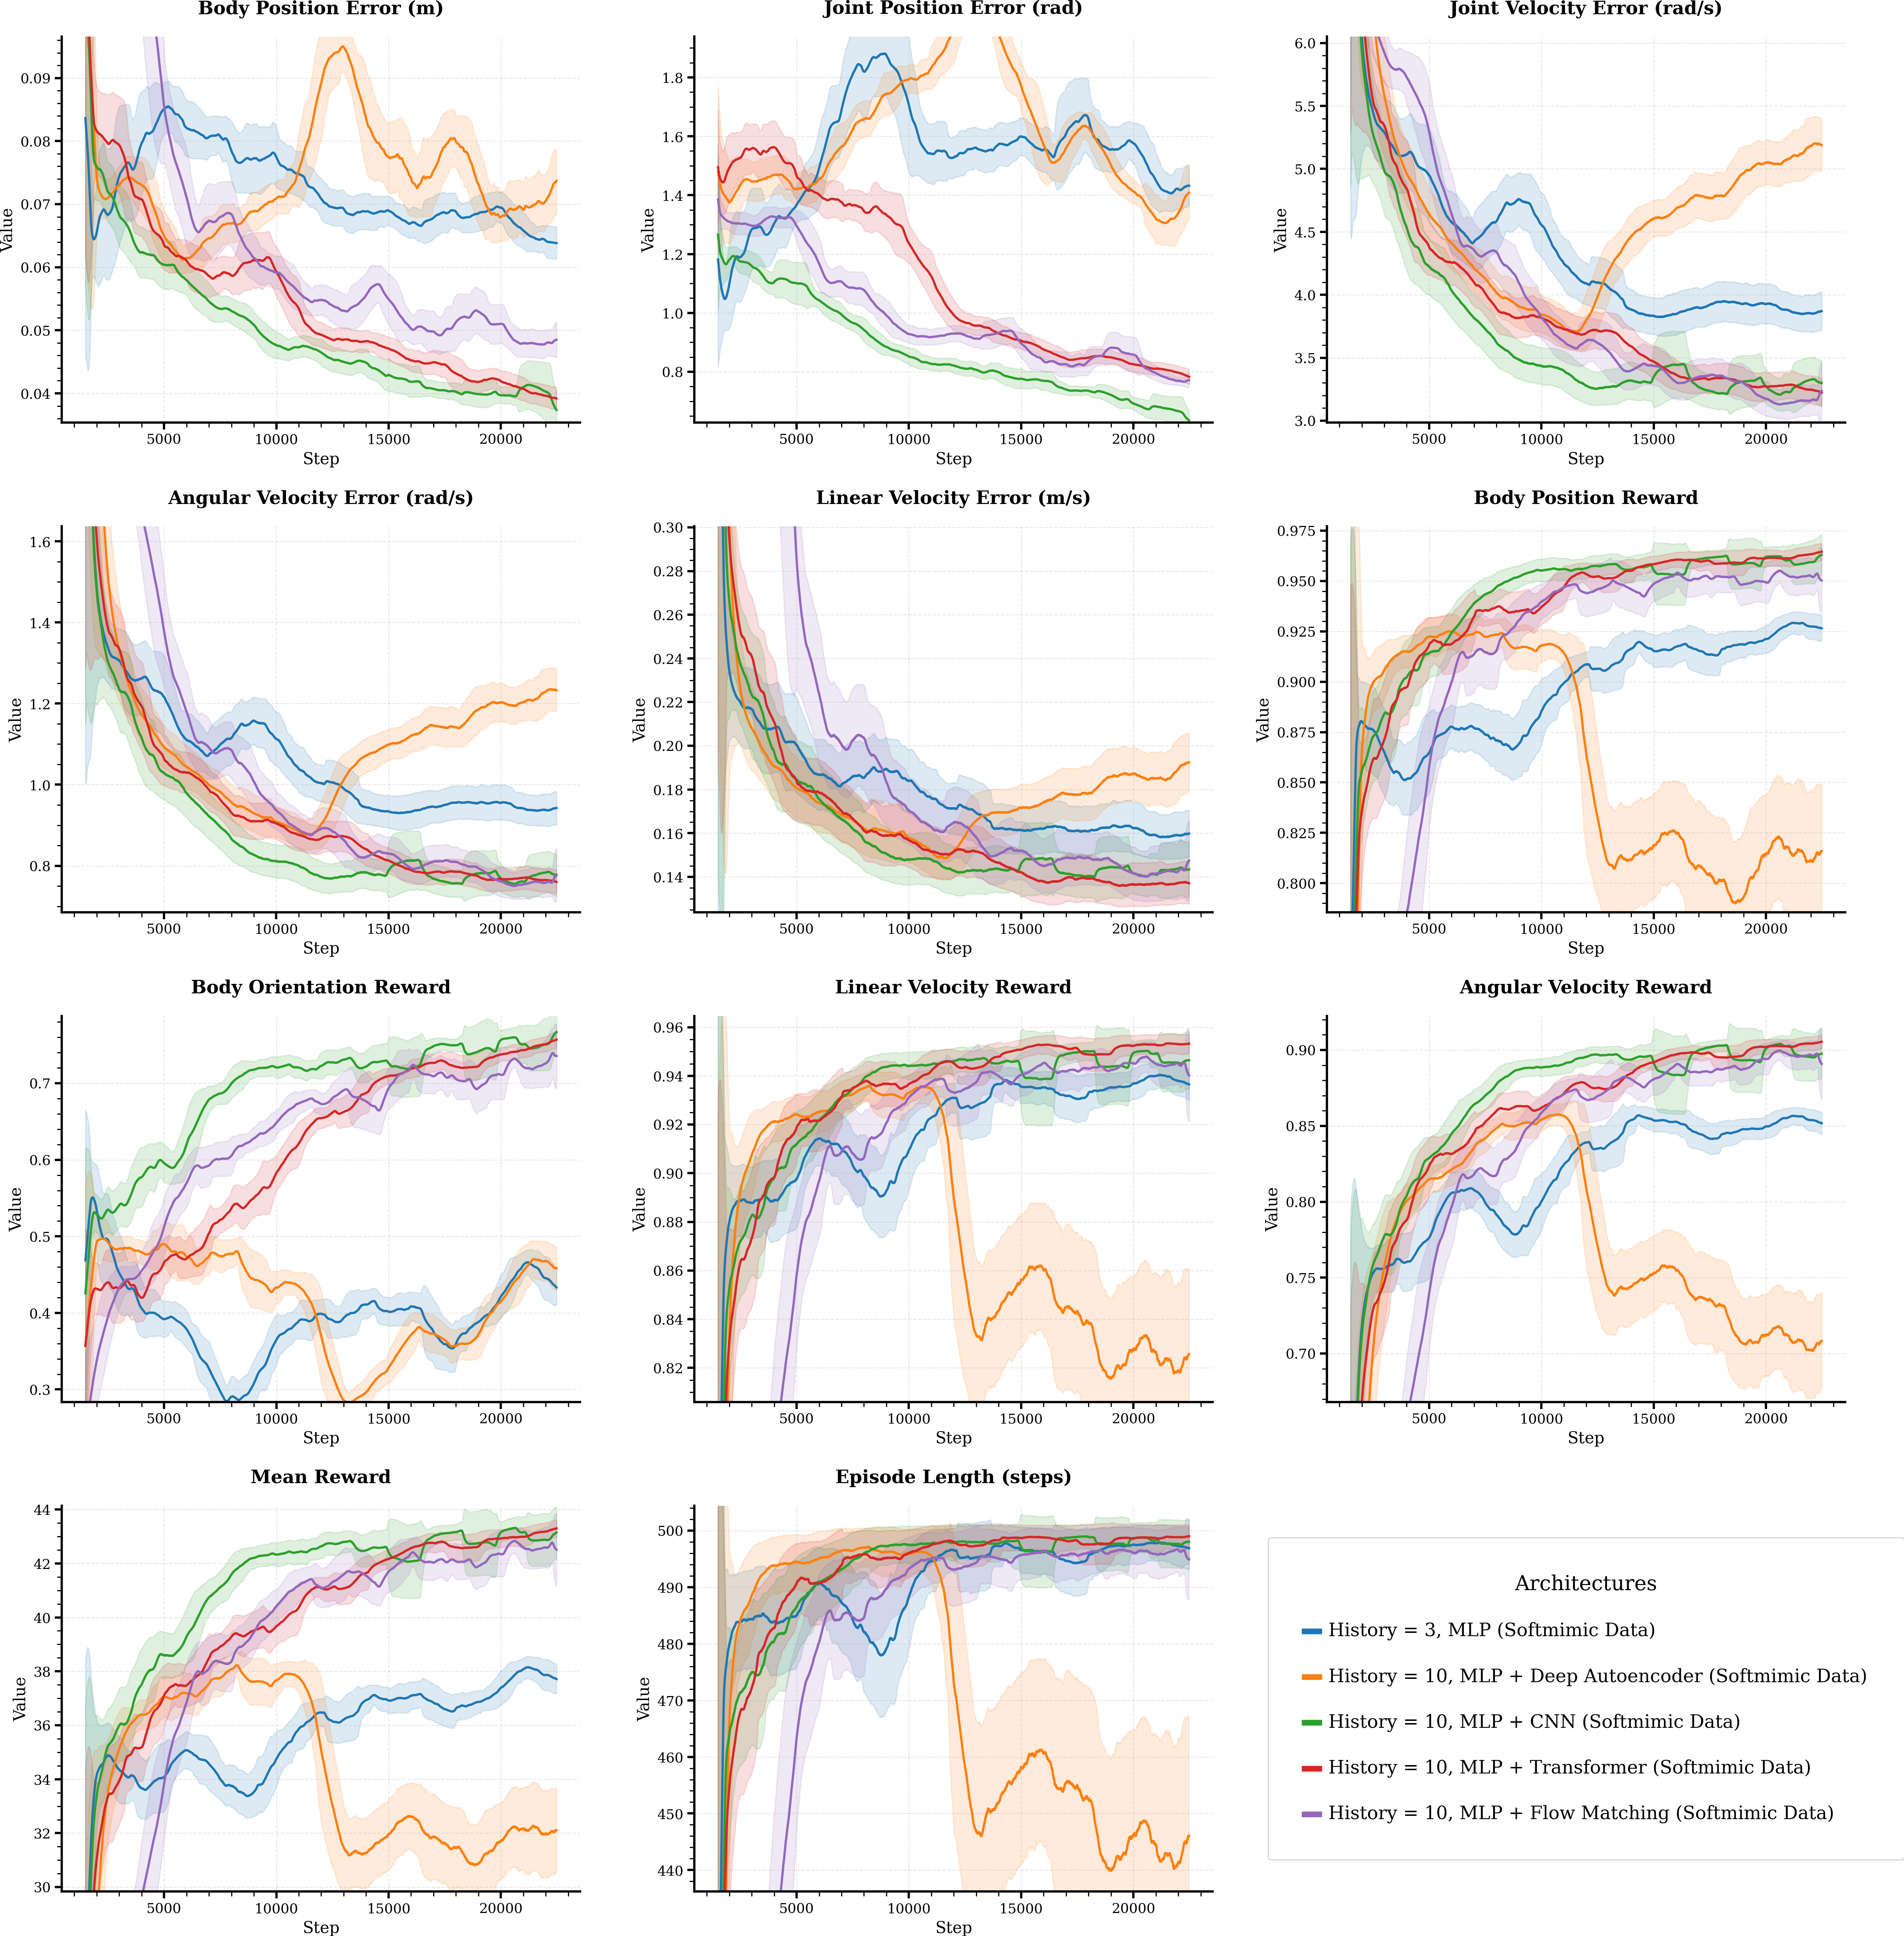
\includegraphics[width=\textwidth]{figure/training_curves.png}
        \captionof{figure}{Training curves for SoftMimic impedance controllers with different history encoders.}
        \label{fig:training-curves}
    \end{minipage}
    \hfill
    \begin{minipage}{0.48\textwidth}
        \centering
        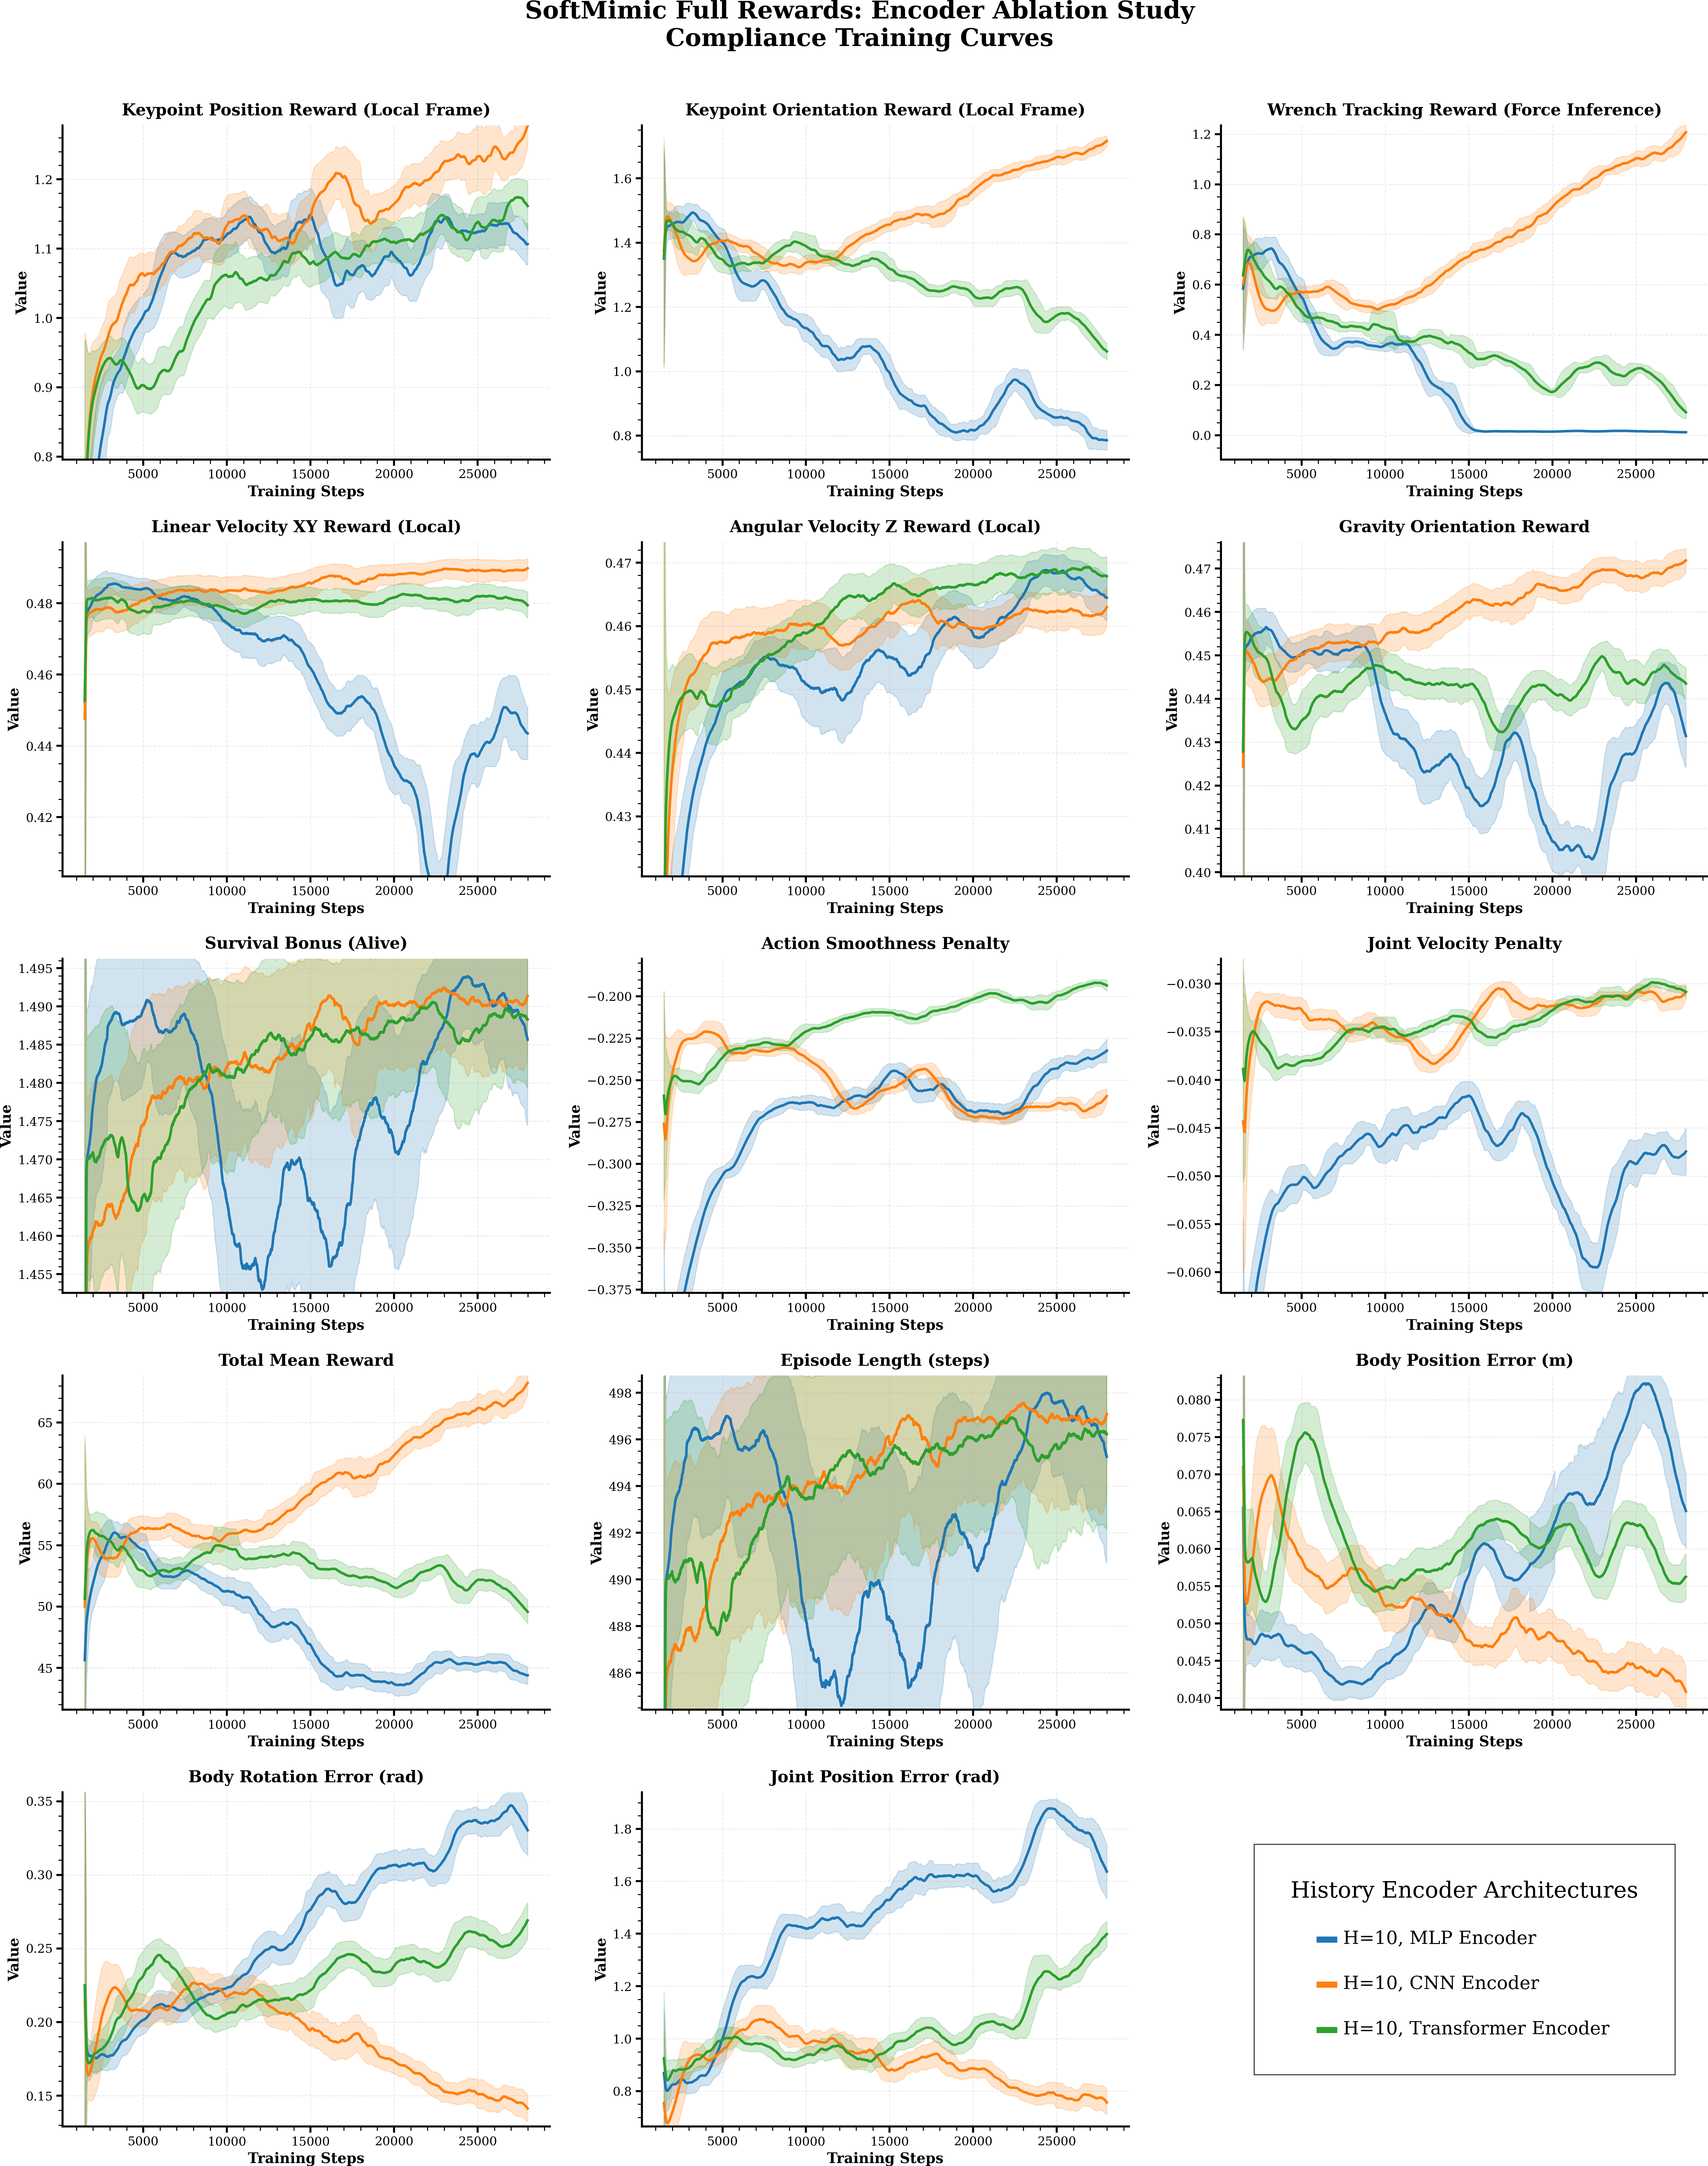
\includegraphics[width=\textwidth]{figure/softmimic_rewards_training_curves.png}
        \captionof{figure}{SoftMimic compliance-training curves on the G1 retargeted LAFAN1 dataset for different history encoders.}
        \label{fig:softmimic-rewards-training-curves}
    \end{minipage}
\end{figure}

\subsection{Training Details and Hyperparameters}
\label{sec:training-details}

We largely follow the SoftMimic training setup \cite{margolis2025softmimiclearningcompliantwholebody}, adapting only the history encoders and observation window length.

\paragraph{Parallel simulation and rollout length.}
All policies are trained in parallel over 4096 simulated environments using MuJoCo. Each PPO update processes rollouts of length $24$ time steps per environment. This choice balances three factors: (i) stable gradient estimates from sufficiently long trajectories, (ii) frequent policy updates for rapid learning, and (iii) manageable GPU/CPU memory usage.

\paragraph{PPO hyperparameters.}
Unless otherwise stated, we use the following PPO settings:
\begin{itemize}
    \item Discount factor $\gamma = 0.99$ and GAE parameter $\lambda = 0.95$, a standard choice for continuous control that favors long-horizon returns while keeping variance reasonable.
    \item Learning rate $1 \times 10^{-3}$ with an adaptive schedule based on a KL-divergence target of $0.01$, allowing the optimizer to automatically reduce the step size as the policy nears convergence.
    \item $5$ optimization epochs per rollout and $4$ minibatches per epoch, yielding $20$ gradient steps per batch.
    \item Clipping range $\epsilon = 0.2$ and maximum gradient norm $1.0$.
    \item Value loss coefficient $c_{\mathrm{vf}} = 1.0$ and entropy coefficient $c_{\mathrm{ent}} = 0.002$.
\end{itemize}
These values closely match the configuration used in prior humanoid control work and have been validated to provide stable training on high-dimensional motion imitation tasks.

\paragraph{Network architectures.}
For the MLP backbone, we use:
\begin{itemize}
    \item Policy head: a multi-layer perceptron with hidden layers of sizes $[512, 512, 256, 128]$ and ELU activations.
    \item Value head: a multi-layer perceptron with hidden layers $[512, 512, 512, 512]$ and ELU activations.
\end{itemize}
The different temporal encoders (MLP, CNN, Transformer, Autoencoder, Flow Matching) produce a fixed-size latent representation of the history and reference, which is then concatenated with the stiffness command and passed to this backbone. We selected these widths to be large enough to capture the complex, high-dimensional dependencies of humanoid motion, while still allowing efficient training with thousands of parallel environments.

For the history-$3$ baseline, we stack three recent observations and feed them directly to the MLP. For the history-$10$ models, the encoders operate on sequences of length $H = 10$. In particular:
\begin{itemize}
    \item The CNN encoder applies several 1D temporal convolutions with small kernel sizes to capture local temporal patterns.
    \item The Transformer encoder uses a modest number of self-attention layers and heads to model longer-range dependencies.
    \item The Autoencoder compresses motion windows into a low-dimensional latent, probing whether a bottleneck improves generalization.
    \item The Flow Matching encoder learns continuous-time trajectory representations that are then pooled into a latent vector.
\end{itemize}
The comparison across these variants is intended to isolate the effect of temporal representation capacity on compliant behavior and gravity-compensation-like responses.

\paragraph{Domain randomization and observation noise.}
To improve robustness and avoid overfitting to a single simulator configuration, we apply moderate domain randomization following \cite{margolis2025softmimiclearningcompliantwholebody}: link masses, joint damping, friction, and ground contact parameters are randomly perturbed within fixed ranges at the beginning of each episode. We also add zero-mean noise to joint positions, joint velocities, base angular velocity, and the projected gravity vector at each time step. The magnitude of these perturbations is chosen so that the resulting noise floor matches typical sensor uncertainty on real humanoid hardware, while remaining small enough to preserve the structure of the reference motions.

\paragraph{Reward weights and design justification.}
The reward design follows three principles:
\begin{enumerate}
    \item \textbf{Compliance should be explicit.} We place relatively high weights on the task-space compliance terms (end-effector position/orientation and force/torque matching) so that the policy is directly incentivized to realize the desired stiffness behavior rather than treating compliance as a side effect.
    \item \textbf{Motion quality must remain high.} Keypoint and base tracking terms use weights of comparable magnitude, ensuring that in the absence of external forces the policy behaves similarly to a standard motion imitation controller and produces visually high-quality trajectories.
    \item \textbf{Safety and smoothness are regularizers, not primary goals.} Alive bonuses, joint limit penalties, velocity and action-rate regularization, and stance foot stability terms have smaller magnitudes. They shape the behavior away from pathological regimes (e.g., saturating torques, foot skating) without overwhelming the main tracking and compliance objectives.
\end{enumerate}
We adopt the same numeric weights as SoftMimic for these terms, which were tuned to satisfy a simple design target: approximate end-effector displacement errors below $10$\,cm and force errors below $15$\,N across most of the stiffness range, while maintaining motion tracking errors comparable to a stiff motion-tracking baseline.

\paragraph{Architectural justification.}
We use the short-history MLP as a strong but standard baseline representative of common humanoid imitation controllers. The longer-history encoders are motivated by the observation that compliant responses and gravity compensation inherently depend on the evolution of disturbances over time. CNNs provide a good trade-off between capacity and efficiency for local temporal patterns; Transformers and Flow Matching encoders can, in principle, represent longer-range dependencies and continuous-time behaviors. Our experiments (Section~\ref{sec:results}) confirm that increasing history length and introducing structured temporal encoders yield substantial gains in stability and compliance, supporting the view that temporal representation is a key design axis for impedance whole-body control.

\subsubsection{Results}

Figure~\ref{fig:softmimic-rewards-training-curves} shows the full SoftMimic compliance-training curves across key rewards and error terms for the main encoder variants, while Figure~\ref{fig:softmimic-histograms-common-iter} compares metrics at a fixed training iteration.

\begin{figure}[H]
    \centering
    \includegraphics[width=0.6\textwidth]{figure/softmimic_rewards_histograms_common_iter.png}
    \caption{Metric comparison for SoftMimic encoders at a common training iteration.}
    \label{fig:softmimic-histograms-common-iter}
\end{figure}

Overall, extending the history window from $H=3$ to $H=10$ and adding a dedicated encoder substantially improves performance.
The longer-history models exhibit faster convergence, higher body/orientation/velocity rewards, and lower body, joint, and velocity errors than the short-history MLP baseline.
Among the $H=10$ variants, the MLP + CNN encoder provides the best quantitative performance: it achieves the highest mean reward and episode length, along with the lowest steady-state errors across most metrics.
The Transformer and Flow Matching encoders closely follow the CNN, while the Autoencoder variant lags and shows more instability during training.

\subsubsection{Analysis and Discussion}

\paragraph{Compliance versus tracking.}
Although the MLP + CNN encoder is quantitatively strongest under our scalar metrics, qualitative rollouts reveal that the Flow Matching encoder produces noticeably more compliant behavior: the robot yields more softly to external pushes and contacts and avoids overly stiff corrections.
This suggests that our current reward shaping and evaluation metrics, which emphasize tight tracking and stability, systematically favor slightly stiffer policies, even when softer, more compliant responses are desirable for safe whole-body interaction.

\paragraph{Impact of history and representation.}
The gains from longer history and structured encoders highlight the importance of temporal representation for compliant whole-body control.
Compliant responses depend not only on the current configuration but also on how disturbances evolve over time.
CNN, Transformer, and Flow Matching encoders all exploit this temporal structure to infer external forces and modulate effective stiffness, whereas the feedforward MLP struggles to maintain both balance and compliant behavior under perturbations.

\paragraph{Limitations from IK-generated references.}
A key limitation exposed by these experiments is the quality of the IK-generated compliant references.
Some augmented trajectories are physically infeasible or demand near-singular configurations and large corrective torques, making them difficult for any policy to reproduce under realistic dynamics.
This manifests as plateaus and residual errors in the training curves and limits the attainable rewards for all encoders.
We therefore view the IK augmentation pipeline as the primary bottleneck in the current SoftMimic setup: improving dynamic feasibility constraints or filtering out problematic references is likely necessary to fully capitalize on richer encoder architectures and to approach true gravity-compensated behavior.

\section{Results and Analysis}
\label{sec:results}

\subsection{Quantitative Results}
Across all tasks and disturbance scenarios, the history-$10$ MLP+CNN encoder consistently attains the highest mean reward, longest episode lengths, and lowest tracking errors.
Compared to the history-$3$ MLP baseline, body position error is reduced, joint and velocity errors decrease, and stability under perturbations improves.
Transformer and Flow Matching encoders achieve nearly comparable performance, confirming that richer temporal modeling is beneficial for impedance behavior.

\subsection{Qualitative Results}
Qualitatively, all longer-history models display more stable and fluid motions than the short-history MLP.
The Flow Matching encoder, in particular, appears more compliant: under pushes and environmental contacts, the robot yields smoothly and settles into new configurations without oscillation.
By contrast, the CNN model, while tracking the reference more tightly, occasionally responds with sharper corrections that feel stiffer.
These observations suggest that quantitative metrics alone do not fully capture the perceived compliance of the behavior.

\subsection{Ablation Studies}
Our encoder ablations indicate that:
\begin{itemize}
    \item Increasing history length from $H=3$ to $H=10$ is critical for learning meaningful impedance responses.
    \item Architectural choices (CNN, Transformer, Flow Matching) provide similar quantitative gains, but have distinct qualitative trade-offs in compliance and smoothness.
    \item Autoencoder-based compression can harm stability, likely due to reconstruction errors obscuring fine-grained motion details important for balance and contact.
\end{itemize}
These findings support the view that gravity-compensated whole-body behavior is a long-horizon problem where temporal representation is central.

\section{Discussion, Limitations, and Future Work}
\label{sec:discussion}

\subsection{Discussion of Findings}
Our experiments show that SoftMimic-style compliant imitation provides a strong basis for impedance whole-body control.
By augmenting reference motions with compliant IK variants and training policies with longer-history encoders, we can realize controllers that are both stable and tunably compliant.
CNN- and Flow-Matching-based architectures are particularly effective, the former excelling in tracking metrics and the latter in qualitative compliance.

\subsection{Limitations}

Despite these promising results, several limitations remain:
\begin{itemize}
    \item \textbf{IK bottleneck.} The physical feasibility of IK-generated compliant references is a major constraint.
    Infeasible or near-singular configurations limit the best achievable performance and may bias the learned controller away from physically plausible impedance behavior.
    \item \textbf{Gravity compensation.} Full gravity-compensated control is not yet implemented.
    Learning such behavior likely requires even longer histories and models that can approximate exponential moving averages of forces over time.
    \item \textbf{Simulation only.} All results are in simulation; real-world deployment will require handling sensor noise, unmodeled dynamics, and safety constraints.
    \item \textbf{Limited task diversity.} We focus on a modest set of reaching, stepping, turning, and simple manipulation tasks; broader evaluation is needed to claim general-purpose whole-body control.
\end{itemize}

\subsection{Future Work}

A natural next step is to combine the compliant impedance controller developed here with large-scale motion datasets and language conditioning.

\paragraph{Towards language-conditioned impedance control.}
Frameworks such as BeyondMimic \cite{liao2025beyondmimicmotiontrackingversatile}, Motion-X++ \cite{zhang2025motionxlargescalemultimodal3d}, and SnapMoGen \cite{guo2025snapmogenhumanmotiongeneration} provide diverse motion data with semantic text labels.
We envision a two-level system in which:
\begin{itemize}
    \item A high-level, language-conditioned model (e.g., trajectory diffusion or flow matching) generates motion plans or tokenized trajectories from text.
    \item The impedance whole-body controller developed in this work executes these plans while ensuring compliance and safety.
\end{itemize}

\paragraph{Modeling and representation.}
Several modeling directions emerge:
\begin{itemize}
    \item \textbf{Hierarchical tokenization.} Introduce a hierarchical tokenization scheme for motion sequences, capturing both coarse high-level structure and fine-grained joint behavior.
    \item \textbf{Variable-time control.} Extend the policy to output both actions and their durations (variable time steps), potentially improving efficiency and expressiveness.
    \item \textbf{Style and weighting spaces.} Different reward weightings induce different behaviors (e.g., more compliant vs.\ more precise).
    Identifying a natural configuration space for these weightings and feeding it as an input to the policy could enable user-controlled style modulation.
    \item \textbf{Structured augmentation.} Apply structured perturbations to reference poses on the input side of the policy to improve robustness and generalization.
\end{itemize}

\paragraph{Scaling and foundation controllers.}
Finally, we aim to:
\begin{itemize}
    \item Scale training to obtain \emph{foundational compliant whole-body controllers}, analogous to recent efforts such as SONIC, but with explicit impedance behavior.
    \item Integrate gravity compensation by using longer histories and architectures that explicitly implement temporal filtering (e.g., recurrent or continuous-time models).
    \item Move from the current two-stage (IK + RL) setup towards more unified single-stage training, potentially with annealed losses that gradually emphasize precision in hand and end-effector poses.
\end{itemize}


\section{Conclusion}
\label{sec:conclusion}

We presented a SoftMimic-based approach to impedance whole-body control for humanoid robots, focusing on compliant behavior and tunable stiffness.
By augmenting reference motions with IK-generated compliant variants and training policies with longer-history encoders, we obtain controllers that track motions accurately while responding more safely to external forces.
Our encoder ablations highlight the importance of temporal representation and reveal trade-offs between quantitative tracking metrics and qualitative compliance.
Although gravity compensation and large-scale language conditioning remain open challenges, the methods and insights developed here provide a principled foundation for future work on compliant, language-driven humanoid control.

%% References
\printbibliography
% \bibliographystyle{plain}
% \bibliography{refs}

\end{document}